
%% bare_conf.tex
%% V1.3
%% 2007/01/11
%% by Michael Shell
%% See:
%% http://www.michaelshell.org/
%% for current contact information.
%%
%% This is a skeleton file demonstrating the use of IEEEtran.cls
%% (requires IEEEtran.cls version 1.7 or later) with an IEEE conference paper.
%%
%% Support sites:
%% http://www.michaelshell.org/tex/ieeetran/
%% http://www.ctan.org/tex-archive/macros/latex/contrib/IEEEtran/
%% and
%% http://www.ieee.org/

%%*************************************************************************
%% Legal Notice:
%% This code is offered as-is without any warranty either expressed or
%% implied; without even the implied warranty of MERCHANTABILITY or
%% FITNESS FOR A PARTICULAR PURPOSE!
%% User assumes all risk.
%% In no event shall IEEE or any contributor to this code be liable for
%% any damages or losses, including, but not limited to, incidental,
%% consequential, or any other damages, resulting from the use or misuse
%% of any information contained here.
%%
%% All comments are the opinions of their respective authors and are not
%% necessarily endorsed by the IEEE.
%%
%% This work is distributed under the LaTeX Project Public License (LPPL)
%% ( http://www.latex-project.org/ ) version 1.3, and may be freely used,
%% distributed and modified. A copy of the LPPL, version 1.3, is included
%% in the base LaTeX documentation of all distributions of LaTeX released
%% 2003/12/01 or later.
%% Retain all contribution notices and credits.
%% ** Modified files should be clearly indicated as such, including  **
%% ** renaming them and changing author support contact information. **
%%
%% File list of work: IEEEtran.cls, IEEEtran_HOWTO.pdf, bare_adv.tex,
%%                    bare_conf.tex, bare_jrnl.tex, bare_jrnl_compsoc.tex
%%*************************************************************************

% *** Authors should verify (and, if needed, correct) their LaTeX system  ***
% *** with the testflow diagnostic prior to trusting their LaTeX platform ***
% *** with production work. IEEE's font choices can trigger bugs that do  ***
% *** not appear when using other class files.                            ***
% The testflow support page is at:
% http://www.michaelshell.org/tex/testflow/



% Note that the a4paper option is mainly intended so that authors in
% countries using A4 can easily print to A4 and see how their papers will
% look in print - the typesetting of the document will not typically be
% affected with changes in paper size (but the bottom and side margins will).
% Use the testflow package mentioned above to verify correct handling of
% both paper sizes by the user's LaTeX system.
%
% Also note that the "draftcls" or "draftclsnofoot", not "draft", option
% should be used if it is desired that the figures are to be displayed in
% draft mode.
%
\documentclass[conference]{IEEEtran}
\usepackage{balance}  % to better equalize the last page
\usepackage{graphics} % for EPS, load graphicx instead
\usepackage{times}    % comment if you want LaTeX's default font
\usepackage{url}      % llt: nicely formatted URLs
\usepackage{multirow}
\usepackage{euscript}
\usepackage{url}
\usepackage{pstricks, pst-node}
\usepackage{textcomp}
\usepackage{stmaryrd}
\usepackage{epsfig}
% \usepackage{subfigure}
\usepackage{booktabs}
\usepackage{graphicx}
\usepackage{float}
\usepackage{tabularx}
\usepackage{epstopdf}


\usepackage{graphicx}
\usepackage{latexsym}
\usepackage[fleqn]{amsmath}
\usepackage[varg]{txfonts}
\usepackage{float}

\usepackage{graphicx, graphics}
\usepackage{algorithmic}
\usepackage{tabularx}
\renewcommand{\algorithmicrequire}{\textbf{Input:}}
\renewcommand{\algorithmicensure}{\textbf{Output:}}

\usepackage{subcaption}
% Add the compsoc option for Computer Society conferences.
%
% If IEEEtran.cls has not been installed into the LaTeX system files,
% manually specify the path to it like:
% \documentclass[conference]{../sty/IEEEtran}


\makeatletter
\newenvironment{tablehere}
  {\def\@captype{table}}
  {}

\newenvironment{figurehere}
  {\def\@captype{figure}}
  {}
\makeatother




% Some very useful LaTeX packages include:
% (uncomment the ones you want to load)


% *** MISC UTILITY PACKAGES ***
%
%\usepackage{ifpdf}
% Heiko Oberdiek's ifpdf.sty is very useful if you need conditional
% compilation based on whether the output is pdf or dvi.
% usage:
% \ifpdf
%   % pdf code
% \else
%   % dvi code
% \fi
% The latest version of ifpdf.sty can be obtained from:
% http://www.ctan.org/tex-archive/macros/latex/contrib/oberdiek/
% Also, note that IEEEtran.cls V1.7 and later provides a builtin
% \ifCLASSINFOpdf conditional that works the same way.
% When switching from latex to pdflatex and vice-versa, the compiler may
% have to be run twice to clear warning/error messages.






% *** CITATION PACKAGES ***
%
%\usepackage{cite}
% cite.sty was written by Donald Arseneau
% V1.6 and later of IEEEtran pre-defines the format of the cite.sty package
% \cite{} output to follow that of IEEE. Loading the cite package will
% result in citation numbers being automatically sorted and properly
% "compressed/ranged". e.g., [1], [9], [2], [7], [5], [6] without using
% cite.sty will become [1], [2], [5]--[7], [9] using cite.sty. cite.sty's
% \cite will automatically add leading space, if needed. Use cite.sty's
% noadjust option (cite.sty V3.8 and later) if you want to turn this off.
% cite.sty is already installed on most LaTeX systems. Be sure and use
% version 4.0 (2003-05-27) and later if using hyperref.sty. cite.sty does
% not currently provide for hyperlinked citations.
% The latest version can be obtained at:
% http://www.ctan.org/tex-archive/macros/latex/contrib/cite/
% The documentation is contained in the cite.sty file itself.






% *** GRAPHICS RELATED PACKAGES ***
%
\ifCLASSINFOpdf
  % \usepackage[pdftex]{graphicx}
  % declare the path(s) where your graphic files are
  % \graphicspath{{../pdf/}{../jpeg/}}
  % and their extensions so you won't have to specify these with
  % every instance of \includegraphics
  % \DeclareGraphicsExtensions{.pdf,.jpeg,.png}
\else
  % or other class option (dvipsone, dvipdf, if not using dvips). graphicx
  % will default to the driver specified in the system graphics.cfg if no
  % driver is specified.
  % \usepackage[dvips]{graphicx}
  % declare the path(s) where your graphic files are
  % \graphicspath{{../eps/}}
  % and their extensions so you won't have to specify these with
  % every instance of \includegraphics
  % \DeclareGraphicsExtensions{.eps}
\fi
% graphicx was written by David Carlisle and Sebastian Rahtz. It is
% required if you want graphics, photos, etc. graphicx.sty is already
% installed on most LaTeX systems. The latest version and documentation can
% be obtained at:
% http://www.ctan.org/tex-archive/macros/latex/required/graphics/
% Another good source of documentation is "Using Imported Graphics in
% LaTeX2e" by Keith Reckdahl which can be found as epslatex.ps or
% epslatex.pdf at: http://www.ctan.org/tex-archive/info/
%
% latex, and pdflatex in dvi mode, support graphics in encapsulated
% postscript (.eps) format. pdflatex in pdf mode supports graphics
% in .pdf, .jpeg, .png and .mps (metapost) formats. Users should ensure
% that all non-photo figures use a vector format (.eps, .pdf, .mps) and
% not a bitmapped formats (.jpeg, .png). IEEE frowns on bitmapped formats
% which can result in "jaggedy"/blurry rendering of lines and letters as
% well as large increases in file sizes.
%
% You can find documentation about the pdfTeX application at:
% http://www.tug.org/applications/pdftex





% *** MATH PACKAGES ***
%
%\usepackage[cmex10]{amsmath}
% A popular package from the American Mathematical Society that provides
% many useful and powerful commands for dealing with mathematics. If using
% it, be sure to load this package with the cmex10 option to ensure that
% only type 1 fonts will utilized at all point sizes. Without this option,
% it is possible that some math symbols, particularly those within
% footnotes, will be rendered in bitmap form which will result in a
% document that can not be IEEE Xplore compliant!
%
% Also, note that the amsmath package sets \interdisplaylinepenalty to 10000
% thus preventing page breaks from occurring within multiline equations. Use:
%\interdisplaylinepenalty=2500
% after loading amsmath to restore such page breaks as IEEEtran.cls normally
% does. amsmath.sty is already installed on most LaTeX systems. The latest
% version and documentation can be obtained at:
% http://www.ctan.org/tex-archive/macros/latex/required/amslatex/math/





% *** SPECIALIZED LIST PACKAGES ***
%
%\usepackage{algorithmic}
% algorithmic.sty was written by Peter Williams and Rogerio Brito.
% This package provides an algorithmic environment fo describing algorithms.
% You can use the algorithmic environment in-text or within a figure
% environment to provide for a floating algorithm. Do NOT use the algorithm
% floating environment provided by algorithm.sty (by the same authors) or
% algorithm2e.sty (by Christophe Fiorio) as IEEE does not use dedicated
% algorithm float types and packages that provide these will not provide
% correct IEEE style captions. The latest version and documentation of
% algorithmic.sty can be obtained at:
% http://www.ctan.org/tex-archive/macros/latex/contrib/algorithms/
% There is also a support site at:
% http://algorithms.berlios.de/index.html
% Also of interest may be the (relatively newer and more customizable)
% algorithmicx.sty package by Szasz Janos:
% http://www.ctan.org/tex-archive/macros/latex/contrib/algorithmicx/




% *** ALIGNMENT PACKAGES ***
%
\usepackage{array}
% Frank Mittelbach's and David Carlisle's array.sty patches and improves
% the standard LaTeX2e array and tabular environments to provide better
% appearance and additional user controls. As the default LaTeX2e table
% generation code is lacking to the point of almost being broken with
% respect to the quality of the end results, all users are strongly
% advised to use an enhanced (at the very least that provided by array.sty)
% set of table tools. array.sty is already installed on most systems. The
% latest version and documentation can be obtained at:
% http://www.ctan.org/tex-archive/macros/latex/required/tools/


%\usepackage{mdwmath}
%\usepackage{mdwtab}
% Also highly recommended is Mark Wooding's extremely powerful MDW tools,
% especially mdwmath.sty and mdwtab.sty which are used to format equations
% and tables, respectively. The MDWtools set is already installed on most
% LaTeX systems. The lastest version and documentation is available at:
% http://www.ctan.org/tex-archive/macros/latex/contrib/mdwtools/


% IEEEtran contains the IEEEeqnarray family of commands that can be used to
% generate multiline equations as well as matrices, tables, etc., of high
% quality.


%\usepackage{eqparbox}
% Also of notable interest is Scott Pakin's eqparbox package for creating
% (automatically sized) equal width boxes - aka "natural width parboxes".
% Available at:
% http://www.ctan.org/tex-archive/macros/latex/contrib/eqparbox/





% *** SUBFIGURE PACKAGES ***
%\usepackage[tight,footnotesize]{subfigure}
% subfigure.sty was written by Steven Douglas Cochran. This package makes it
% easy to put subfigures in your figures. e.g., "Figure 1a and 1b". For IEEE
% work, it is a good idea to load it with the tight package option to reduce
% the amount of white space around the subfigures. subfigure.sty is already
% installed on most LaTeX systems. The latest version and documentation can
% be obtained at:
% http://www.ctan.org/tex-archive/obsolete/macros/latex/contrib/subfigure/
% subfigure.sty has been superceeded by subfig.sty.



% \usepackage{caption}
%\usepackage[font=footnotesize]{subfig}
% subfig.sty, also written by Steven Douglas Cochran, is the modern
% replacement for subfigure.sty. However, subfig.sty requires and
% automatically loads Axel Sommerfeldt's caption.sty which will override
% IEEEtran.cls handling of captions and this will result in nonIEEE style
% figure/table captions. To prevent this problem, be sure and preload
% caption.sty with its "caption=false" package option. This is will preserve
% IEEEtran.cls handing of captions. Version 1.3 (2005/06/28) and later
% (recommended due to many improvements over 1.2) of subfig.sty supports
% the caption=false option directly:
%\usepackage[caption=false,font=footnotesize]{subfig}
%
% The latest version and documentation can be obtained at:
% http://www.ctan.org/tex-archive/macros/latex/contrib/subfig/
% The latest version and documentation of caption.sty can be obtained at:
% http://www.ctan.org/tex-archive/macros/latex/contrib/caption/




% *** FLOAT PACKAGES ***
%
%\usepackage{fixltx2e}
% fixltx2e, the successor to the earlier fix2col.sty, was written by
% Frank Mittelbach and David Carlisle. This package corrects a few problems
% in the LaTeX2e kernel, the most notable of which is that in current
% LaTeX2e releases, the ordering of single and double column floats is not
% guaranteed to be preserved. Thus, an unpatched LaTeX2e can allow a
% single column figure to be placed prior to an earlier double column
% figure. The latest version and documentation can be found at:
% http://www.ctan.org/tex-archive/macros/latex/base/



%\usepackage{stfloats}
% stfloats.sty was written by Sigitas Tolusis. This package gives LaTeX2e
% the ability to do double column floats at the bottom of the page as well
% as the top. (e.g., "\begin{figure*}[!b]" is not normally possible in
% LaTeX2e). It also provides a command:
%\fnbelowfloat
% to enable the placement of footnotes below bottom floats (the standard
% LaTeX2e kernel puts them above bottom floats). This is an invasive package
% which rewrites many portions of the LaTeX2e float routines. It may not work
% with other packages that modify the LaTeX2e float routines. The latest
% version and documentation can be obtained at:
% http://www.ctan.org/tex-archive/macros/latex/contrib/sttools/
% Documentation is contained in the stfloats.sty comments as well as in the
% presfull.pdf file. Do not use the stfloats baselinefloat ability as IEEE
% does not allow \baselineskip to stretch. Authors submitting work to the
% IEEE should note that IEEE rarely uses double column equations and
% that authors should try to avoid such use. Do not be tempted to use the
% cuted.sty or midfloat.sty packages (also by Sigitas Tolusis) as IEEE does
% not format its papers in such ways.





% *** PDF, URL AND HYPERLINK PACKAGES ***
%
%\usepackage{url}
% url.sty was written by Donald Arseneau. It provides better support for
% handling and breaking URLs. url.sty is already installed on most LaTeX
% systems. The latest version can be obtained at:
% http://www.ctan.org/tex-archive/macros/latex/contrib/misc/
% Read the url.sty source comments for usage information. Basically,
% \url{my_url_here}.





% *** Do not adjust lengths that control margins, column widths, etc. ***
% *** Do not use packages that alter fonts (such as pslatex).         ***
% There should be no need to do such things with IEEEtran.cls V1.6 and later.
% (Unless specifically asked to do so by the journal or conference you plan
% to submit to, of course. )


% correct bad hyphenation here
\hyphenation{op-tical net-works semi-conduc-tor}


\begin{document}
\title{An Empirical Analysis for Automatic Evaluation of Generative Dialogue Systems}

\author{
\IEEEauthorblockN{Cong Feng$^{1,2}$, Wenge Rong$^{1,2}$, Shijie Zhou$^{1,2}$, Jianfei Zhang$^{1,2}$, Zhang Xiong$^{1,2}$}
\IEEEauthorblockA{
	$^{1}$State Key Laboratory of Software Development Environment, Beihang University, Beijing 100191, China\\
	$^{2}$School of Computer Science and Engineering, Beihang University, Beijing 100191, China\\
\{congfeng, w.rong, zhoushijie, zhangjf, xiongz\}@buaa.edu.cn}
}

\maketitle

\begin{abstract}
Evaluating generative dialogue systems with automatic metrics is a challenging task.
It has been shown that word-overlap metrics such as BLEU and word-embedding metrics do not correlate well with human judgements.
In this research, we further show that the scores of these metrics do not correlate well with themselves, which means fine-tuning a dialogue system on one set of metrics may yield inconsistency when testing with another set of metrics.
To better utilize metrics in evaluation, we offer several pragmatic suggestions on the use of automatic metrics to avoid the issue of metric inconsistency by empirically evaluating a set of automatic evaluation metrics.
\end{abstract}

\begin{IEEEkeywords}
% Adjust order by length.
Chatbot, Automatic Metrics, Dialogue Response Generation
\end{IEEEkeywords}

\section{Introduction}
Recently the chat-oriented dialogue systems have seen a boom in the community.
These systems are trained to make an appropriate response given a conversational context and can be applied to various applications.
One of the fundamental techniques in such dialogue systems is the generative model, which can learn language patterns and extract knowledge from the corpus in an unsupervised manner.
The research community has made steady progress with the generative models and one of the most widely applied techniques is the Seq2Seq model \cite{Seq2Seq}.
Although generative models have shown promising results, they incline to give meaningless responses to the questions, e.g., \textit{I don't know}.
The vast space of possibly valid responses also makes their evaluation an open problem \cite{HowNot}.

Currently, most generative dialogue systems are evaluated by borrowing automatic metrics from other tasks, e.g., machine translation, such as BLEU \cite{BLEU}, METEOR \cite{METEOR}, etc.
However, the correlations between these borrowed metrics and human judgements are unclear and researchers generally fall back to human evaluation for better accuracy and reliability \cite{VHRED,Shang}.
It is revealed that those metrics only correlate weakly with human judgements on the non-technical Twitter Corpus and not at all on the technical Ubuntu Dialogue Corpus \cite{HowNot}, calling for new automatic metrics that are more relevant to human judgements.

% 'without human evaluation' is deleted since I want to make it a future work.
In this paper, we follow the previous work and further analyze the behaviors of automatic metrics using different models and datasets. 
We analyze both system-level scores and example-level scores to investigate correlations between different metrics.
The experiments show that the system-level scores generally have better pairwise correlations than that of the example-level scores.
% TODO: correlation of system scores in table.
To reveal possible inconsistencies of the example-level scores,
We further analyze them by sampling the pool of examples (i.e., $(context, resposne, reference)$ tuples) and clustering the metrics using their pairwise correlations as the distance function.
As a result, hierarchical clusters of metrics are observed and common clusters arise across different model-dataset configurations,
which indicates some metrics tend to have higher pairwise correlations than others.

According to the experiment results, it is argued that the example-level scores given by different metrics can be potentially quite inconsistent.
For example, one example may be scored higher than the other under BLEU or other word-overlap metrics, but may get a lower score under an embedding-based metrics.
% TODO: change this.
Therefore, it is strongly recommended to choose consistent metrics for the ease of comparison across different configurations.

The rest of the paper is organized as follows: Section II will present the related work in the literature about the evaluation metrics on dialogue systems.
Section III will illustrate the empirical study's setup and configurations and Section IV will present and discuss the results.
Section V will conclude the paper and point out potential future directions.

\section{Related Work}
In dialogue response generation, to address the issue of low metric-human correlation, various semantic-based methods have been proposed.
For example, the ADEM metric proposed models the human judgements with a feed-forward neural network \cite{ADEM}.
The RUBER metric takes an asymmetric approach w.r.t the response-context pair and response-reference pair, where the former is modeled by a neural network and the latter is measured by an embedding-based metric.
They combined two scores with various heuristics and achieved improvements on a Chinese corpus \cite{RUBER}.
In brief, correlation with human judgements has been the supervised signal guiding the evolution of automatic metrics.

Other popular metrics include perplexity, which is generally used to evaluate statistical language models.
Vinyals et al. revealed that their Seq2Seq dialogue model achieved a much lower perplexity than the n-gram baseline, but they also admitted the drawbacks of using such a metric \cite{GoogleChatbot}.
Serban et al. also used perplexity to evaluate their models \cite{HRED}, along with other metrics.
However they were also not clear about how well these metrics accounted for the grammatical correctness and semantic coherence of the responses.

Generally, automatic metrics have been constantly doubted of their capability to reflect human judgements.
In one of the earliest attempts to the response generation problem, Ritter et al. made an initial examination on the suitability of BLEU to this field leveraging the human data they collected \cite{Ritter11}.
They found that the BLEU scores were very low even on the system level and the correlation was modest.
Similarly, Shang et al. also argued that BLEU did not apply as the reasonable responses evaluation \cite{Shang}.

An extensive study of metric-human correlation was conducted by Liu et al. \cite{HowNot}.
It was revealed that although these metrics could distinguish state-of-art models from baseline models, none of them correlated highly with human scores.
Their work has left us two questions: 1) How can we improve the metric-human correlation? 2) Why do the existing metrics correlate badly with human judgements?
Previous works that proposed enhanced metrics endeavored to answer the first question, while we try to shed some light on the second one.
In particular, we are curious about what can we learn when scores from different metrics are put together and compared across various configurations.

\section{Experiment Configurations}
We train multiple generative models on multiple datasets, and then score the outputs of different model-dataset configurations with various automatic metrics.
Constrained by time and resource, we limit our scope to three commonly used generative models and three datasets.

% ------------------------- %
% --------- Metrics ------- %
% ------------------------- %
\subsection{Metrics}
Here are a list of popular metrics used in dialogue response evaluation included in this research.

1) BLEU \cite{BLEU} is a classical metric for machine translation that reports a high correlation with human scores on the system level.
It owes the quality of a hypothesis to its similarity to multiple references.
It computes the geometric mean of consecutive orders of n-gram precision, multiplied by a brevity penalty.

2) METEOR \cite{METEOR} is a metric proposed to address several issues with BLEU.
It applies multiple stages of unigram matching to the hypothesis and reference, each using a different criterion, such as exact matching, WordNet synonyms, and paraphrases.
An alignment is then created from these unigram matches.
The score is based on the F1 of the alignment and a penalty to shorter matches.

3) ROUGE \cite{ROUGE} is a family of metrics for automatic summarization.
It is based on the F1 score and can integrate different counting units, e.g., n-gram statistics and the longest common subsequence.

4) Embedding Average is a metric based on word embedding, a distributed approach to the meaning of words \cite{word2vec}.
The embedding of a sentence is defined as the average of the embeddings of its composing words.
The similarity of two sentences is then simply defined as the cosine of the corresponding vectors.

5) Vector Extrema \cite{Vector_Extrema} composes the sentence embedding by taking the most extreme value (either maximum or minimum) along each dimension from its constitutive words.
The intuition is that in the embedding space, common words like function words are pulled towards the origin as they appear in the context of many different words, while informative words are pushed away from the origin in either positive or negative direction, since they tend to appear in more specific context.

6) Greedy Matching \cite{GreedyAndOptimal} is an embedding-based method without calculating a sentence vector.
Instead, two sentences under comparison are treated as a weighted bipartite graph, taking their words as nodes and the embedding cosine of two words $\cos(w, w')$ as the edge weight.
The metric is based on a greedy method to solve the optimal matching problem on the weighted graph:
\begin{align}
    G(r, \hat{r}) = \frac{
    \sum_{w \in r} \max_{\hat{w} \in \hat{r}} \cos(e_w, e_{\hat{w}})
    }{ |r| } \\
    \textit{Greedy-Matching} = \frac{
    G(r, \hat{r}) + G(\hat{r}, r)
    }{2}
\end{align}
where $r$ and $\hat{r}$ are the reference and response, respectively.

7) ADEM \cite{ADEM} is an approach based on a concise nueral network.
The model first embeds a context $c$, response $\hat{r}$, and reference $r$ into a low-rank vector space and then predicts the human score with a linear combination of the input features:
\begin{align}
    s(c, r, \hat{r}) = \frac{(c^T M \hat{r} + r^T N \hat{r} - \alpha)}{\beta}
\end{align}
$M, N$ are learnable parameters of the network and $\alpha, \beta$ are constants to normalize the output to a five-point score.
The model is trained on a human-annotated conversation corpus to minimize the squared error with L2 regularization:
\begin{align}
    L = \sum_{i=1}^{K} (s_i - h_i)^2 + \gamma \left\| \theta \right\| _2
\end{align}
where $K$ is the number of samples in a batch.
$s_i$ and $h_i$ are the model prediction and the human score, respectively.
$\theta$ is the parameters of the network and $\gamma$ is the regularization factor.

8) Distinct-N \cite{MMI} measures the rate of unique n-grams in a sentence.
For a sentence, it is the number of unique n-grams divided by the total number of n-grams.
It is a token-level measurement of the diversity of a response.

% ------------------------- %
% --------- Models -------- %
% ------------------------- %
\subsection{Models}
In this research, three representative models from \cite{VHRED} are selected, namely LSTM, HRED, and VHRED. LSTM is a simple model based on the Long Short-Term Memory \cite{LSTM}.
HRED extends the standard Seq2Seq framework by using a hierarchical encoder.
VHRED is an extension to HRED that injects randomness into the decoder to achieve higher diversity.
As such, they form a hierarchy of architectural sophistication and are ideal baselines of generative models.

1) The LSTM model is a simple generative model with a single RNN acting as both an encoder and a decoder.
Note that the generative LSTM model is not autoregressive as the output of the previous time step does not become the input of the current time step.

2) The HRED model \cite{hred-qs,HRED} features a hierarchical encoding mechanism that takes into account the structure of dialogues.
It first encodes each sentence with the \emph{utterance encoder} into a fixed-length utterance vector $e_u$. Then, the utterance vectors are processed iteratively by the \emph{context encoder} to produce a fixed-length context vector $e_d$.
Finally, the \emph{utterance decoder} takes the context vector and generates the next utterance of the dialogue.

3) The VHRED model \cite{VHRED} extends the HRED model with a variational inference mechanism.
Essentially, VHRED injects into the utterance decoder random variables that are sampled from a high-dimension normal distribution, the parameters of which are conditioned on the context vector $e_d$.

The model configurations for utterance encoder, context encoder and utterance decoder are listed in Tables~
\ref{tab:ParametersOfUtteranceEncoder},
\ref{tab:ParametersOfContextEncoder},
\ref{tab:RNNTypeOfUtteranceDecoder}, and
\ref{tab:HiddenUnitsOfUtteranceDecoder},
respectively.
Our model configurations are largely aligned with \cite{VHRED}.
We use the Adam optimizer \cite{AdamOpt} and apply gradient clipping with a threshold of 1.
The learning rate is set to 0.0002 on the Ubuntu Dialogue Corpus and 0.0002 on the other datasets.
All the models are trained on a Nvidia GTX for at least one week.
We use random sampling to generate each example at the time of testing.
\begin{table}[htb]
    \centering
    \caption{Model Configurations}
    \label{tab:model_config}
    \begin{subtable}{0.5\textwidth}
        \centering
        \caption{Utterance Encoder}
        \begin{tabular}{|l|r|r|}
            \hline
            & {\#Embedding} & {\#Hidden Units} \\
            \hline
            LSDSCC & 400 & 1000 \\
            \hline
            OpenSubtitles & 400 & 1000 \\
            \hline
            Ubuntu & 300 & 500 \\
            \hline
        \end{tabular}
    \end{subtable}%
    \begin{subtable}{0.45\textwidth}
        \centering
        \caption{Context Encoder}
        \begin{tabular}{|r|r|}
            \hline
            RNN Direction & \#Hidden Units \\
            \hline
            bidirectional & 1000 \\
            \hline
            bidirectional & 1000 \\
            \hline
            unidirectional & 1000 \\
            \hline
        \end{tabular}
    \end{subtable}
    \begin{subtable}{\textwidth}
        \centering
        \caption{Utterance Decoder}
        \begin{tabular}{|l|*{7}{r|}}
            \hline
            & \multicolumn{3}{c|}{RNN Type}
            & \multicolumn{3}{c|}{\#Hidden Units} \\
            \hline
            & HRED & LSTM & VHRED & HRED & LSTM & VHRED \\
            \hline
            LSDSCC & LSTM & GRU & GRU & 1000 & 2000 & 1000 \\
            \hline
            OpenSubtitles & LSTM & GRU & GRU & 1000 & 2000 & 1000 \\
            \hline
            Ubuntu & LSTM & LSTM & LSTM & 500 & 2000 & 500 \\
            \hline
        \end{tabular}
    \end{subtable}
\end{table}

% --------------------------- %
% --------- Datasets -------- %
% --------------------------- %
\subsection{Datasets}
In this research, we select three commonly used datasets.
The statistics of the training set and testing set are listed in Tables~
\ref{tab:StatisticsOfTrainingSet} and
\ref{tab:StatisticsOfTestingSet}, respectively.
These datasets represent three common domains in the literature, namely technical support, movie subtitles and online forums.
\begin{table}[h]
    \centering
    \caption{Statistics of Training Set}
    \label{tab:StatisticsOfTrainingSet}
    \begin{tabular}{|l|*{4}{c|}}
        \hline
        Dataset & Vocab & \#Samples & \#Tokens & Turns \\
        \hline
        Ubuntu & 20000 & 448833 & 45697699 & multiple \\
        \hline
        OpenSubtitles & 23876 & 11771393 & 379346841 & multiple \\
        \hline
        LSDSCC & 35008 & 738095 & 32355628 & single \\
        \hline
    \end{tabular}
\end{table}

\begin{table}[h]
    \centering
    \caption{Statistics of Testing Set}
    \label{tab:StatisticsOfTestingSet}
    \begin{tabular}{|l|*{2}{c|}}
        \hline
        Dataset & \#Samples & \#Tokens \\
        \hline
        Ubuntu & 18920 & 2045082   \\
        \hline
        OpenSubtitles & 14714 & 474074 \\
        \hline
        LSDSCC & 299 & 10914 \\
        \hline
    \end{tabular}
\end{table}


1) The Ubuntu Dialogue Corpus \cite{ubuntu_corpus} is a large-scale multi-turn dyadic technical corpus collected from the Ubuntu channel of an IRC network\footnote{\url{https://irclogs.ubuntu.com/}}.
It contains a lot of technical symbols, such as filesystem paths, commands, and URLs.

2) The OpenSubtitles dataset \cite{opensub} is an enormous corpus of movie subtitles.
It is collected by the OPUS project \cite{OPUS} from the opensubtitles website\footnote{\url{http://www.opensubtitles.org}}.
Typically, two consecutive utterances are treated as a context-response pair, as in \cite{GoogleChatbot,MMI}.

3) LSDSCC \cite{LSDSCC} is a domain-specific conversation corpus collected from the movie subreddit of the Reddit forum\footnote{\url{https://www.reddit.com/r/datasets}}.
It is believed that a more specific domain can help avoid generating universal responses \cite{LSDSCC}.


\section{Experimental Result and Discussion}
\subsection{System-Level Scores}
We first measured the system-level scores for all configurations, listed in Table~\ref{tab:system_scores} (scores in bold are the best among the three models).
For metrics that do not have an explicit system-level definition, we took the arithmetic average of their example-level scores.
\begin{table*}[htb]
    \centering
    \caption{System-Level Scores}
    \small
    \label{tab:system_scores}
    \setlength{\tabcolsep}{0.09cm}
    \begin{tabular}{|l|r|r|r|r|r|r|r|r|r|}
        \hline
        & \multicolumn{3}{c|}{LSDSCC} & \multicolumn{3}{c|}{OpenSubtitles} & \multicolumn{3}{c|}{Ubuntu}\\
        \hline
        & HRED & LSTM & VHRED & HRED & LSTM & VHRED & HRED & LSTM & VHRED\\
        \hline
        ADEM & \textbf{2.6178} & 2.6127 & 2.6163 & \textbf{2.6228} & 2.6224 & 2.6219 & 2.6353 & \textbf{2.6381} & 2.635\\\hline
        BLEU{-}1 & \textbf{0.08} & 0.0726 & 0.0722 & 0.0672 & 0.0638 & \textbf{0.0753} & 0.1314 & 0.1303 & \textbf{0.1365}\\\hline
        BLEU{-}2 & \textbf{0.0264} & 0.0181 & 0.0185 & 0.0171 & 0.0153 & \textbf{0.0264} & 0.0362 & 0.0345 & \textbf{0.0375}\\\hline
        BLEU{-}3 & \textbf{0.0105} & 0.0052 & 0.0066 & 0.0062 & 0.0055 & \textbf{0.0146} & \textbf{0.009} & 0.007 & 0.0089\\\hline
        BLEU{-}4 & \textbf{0.0053} & 0.0 & 0.0028 & 0.0024 & 0.0022 & \textbf{0.01} & \textbf{0.0029} & 0.0018 & 0.0025\\\hline
        Distinct{-}1 & \textbf{0.9577} & 0.9441 & 0.9558 & \textbf{0.973} & 0.9714 & 0.9714 & 0.9074 & \textbf{0.9257} & 0.9113\\\hline
        Distinct{-}2 & \textbf{0.8541} & 0.8511 & 0.8497 & \textbf{0.8669} & 0.8594 & 0.8665 & \textbf{0.9013} & 0.8603 & 0.8968\\\hline
        Greedy & \textbf{0.3303} & 0.3292 & 0.3267 & 0.3102 & 0.2998 & \textbf{0.3145} & \textbf{0.2775} & 0.2364 & 0.273\\\hline
        Average & \textbf{0.5532} & 0.5467 & 0.5483 & 0.5453 & 0.5295 & \textbf{0.5485} & \textbf{0.574} & 0.5205 & 0.5655\\\hline
        Extrema & \textbf{0.2841} & 0.2835 & 0.2814 & 0.3009 & 0.2929 & \textbf{0.3061} & \textbf{0.29} & 0.2663 & 0.2875\\\hline
        METEOR & \textbf{0.0296} & 0.0258 & 0.0281 & 0.0248 & 0.0233 & \textbf{0.0271} & 0.1657 & 0.1635 & \textbf{0.166}\\\hline
        ROUGE{-}1 & \textbf{0.108} & 0.083 & 0.0978 & 0.0784 & 0.075 & \textbf{0.0872} & 0.1644 & \textbf{0.1836} & 0.1683\\\hline
        ROUGE{-}2 & \textbf{0.0226} & 0.0049 & 0.0081 & 0.0053 & 0.0043 & \textbf{0.0107} & 0.0128 & \textbf{0.0143} & 0.0128\\\hline
        ROUGE{-}3 & \textbf{0.0057} & 0.0002 & 0.0035 & 0.0011 & 0.0009 & \textbf{0.0053} & \textbf{0.0007} & 0.0003 & 0.0005\\\hline
        ROUGE{-}4 & 0.0011 & 0.0 & \textbf{0.003} & 0.0002 & 0.0002 & \textbf{0.0038} & \textbf{0.0002} & 0.0 & 0.0001\\\hline
        ROUGE{-}L & \textbf{0.0956} & 0.0681 & 0.0846 & 0.0742 & 0.0707 & \textbf{0.0826} & 0.1493 & \textbf{0.1722} & 0.1535\\\hline
        ROUGE{-}W & \textbf{0.0792} & 0.0537 & 0.07 & 0.066 & 0.0629 & \textbf{0.0734} & 0.1205 & \textbf{0.1391} & 0.1236\\\hline
        PPL & \textbf{32.5599} & 32.9229 & 37.7149 & 41.6392 & 34.2724 & \textbf{33.6867} & \textbf{39.178} & 46.4061 & 40.2641\\\hline
        \#words & 13.1605 & 14.0067 & 12.3612 & 8.807 & 8.6394 & 8.7798 & 23.0646 & 16.4905 & 21.2449\\
        \hline
    \end{tabular}
\end{table*}


The system-level scores of different metrics look quite consistent in terms of the best performing model on a certain dataset.
For instance, on LSDSCC, the HRED model beats all the other models on all but one metrics (ROUGE-4).
On OpenSubtitles, the VHRED model wins the best of most of the metrics.
On Ubuntu Dialogue Corpus, it is less cleared which one is the best model since the dataset is much more noisy,
but still half of the metrics agree that the HRED model is the best.
The system-level scores are largely consistent in terms of the best performing model.

% TODO: system correlation
However, the consistency among the metrics does not necessarily lead to a high correlation with human judgement, as shown in \cite{HowNot}.
Moreover, since the system-level score is calculated by accumulating over the example-level scores,
it is possible that the inconsistency on the example-level is hidden away.
To reveal the possible inconsistency, we perform analyses on the example-level scores.

\subsection{Example-Level Scores}
On the example level, a matrix $M \in R^{N \times M}$ is calculated for each model instance, where $N$ is the number of examples and $M$ is the number of metrics.
Each row $r_i$ of the matrix is the scores of all metrics for an example $e_i$, while each column $c_j$ is the values of a metric $s_j$ computed for all examples.
All the metrics share the same set of examples within a matrix.
Thus, the correlation of any two columns $c_i, c_j$ can be understood as to how much the corresponding metrics $s_i, s_j$ agree on their shared examples.
We compute the pairwise correlations of the metrics and highlight the degree of correlation with heatmaps, as shown in Fig.~\ref{fig:corr_heatmap}.
We used Pearson's r and all the results are statistically significant.

\begin{figure}[htbp]
    \centering
    \begin{subfigure}{0.33\linewidth}
        \centering
        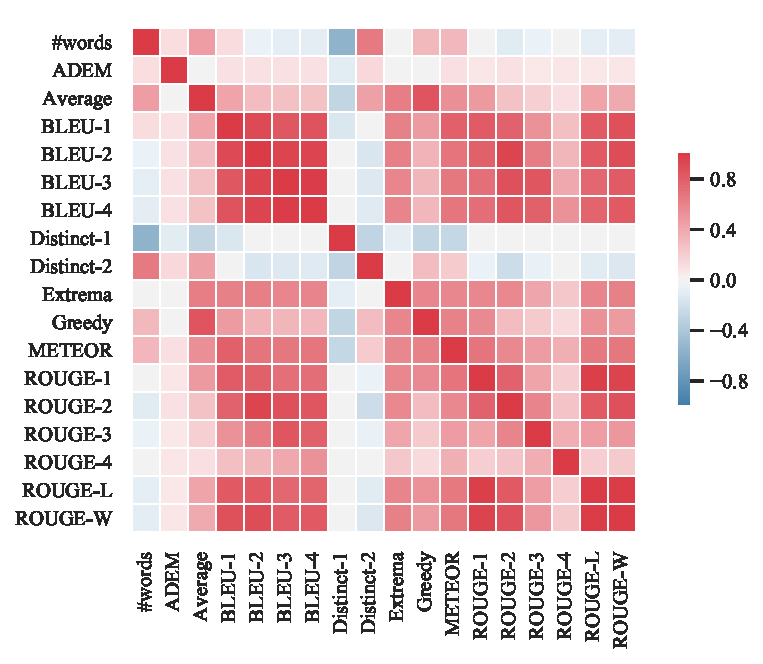
\includegraphics[width=\linewidth]{figure/plot/heatmap/v4/pearson/hred/lsdscc/plot.pdf}
        \caption{(HRED, LSDSCC)}
    \end{subfigure}%
    \begin{subfigure}{0.33\linewidth}
        \centering
        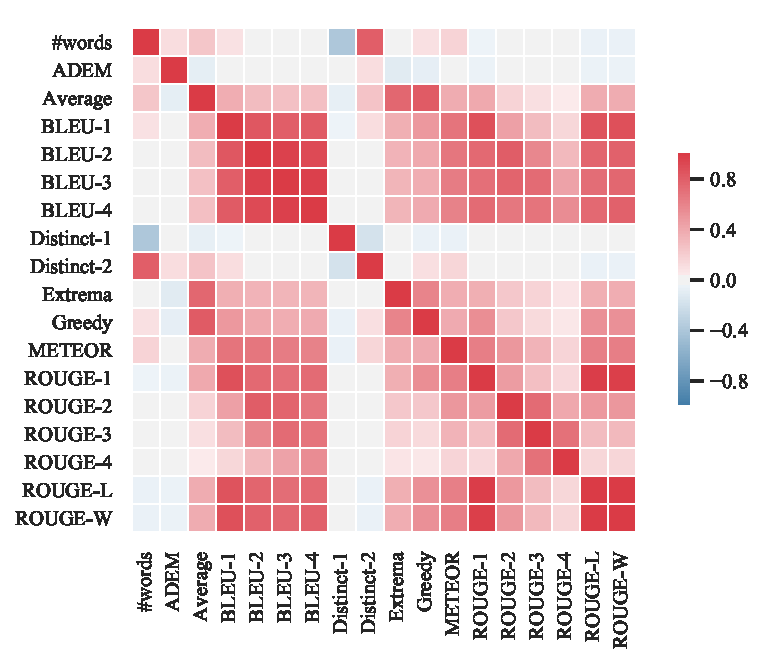
\includegraphics[width=\linewidth]{figure/plot/heatmap/v4/pearson/hred/opensub/plot.pdf}
        \caption{(HRED, OpenSubtitles)}
    \end{subfigure}%
    \begin{subfigure}{0.33\linewidth}
        \centering
        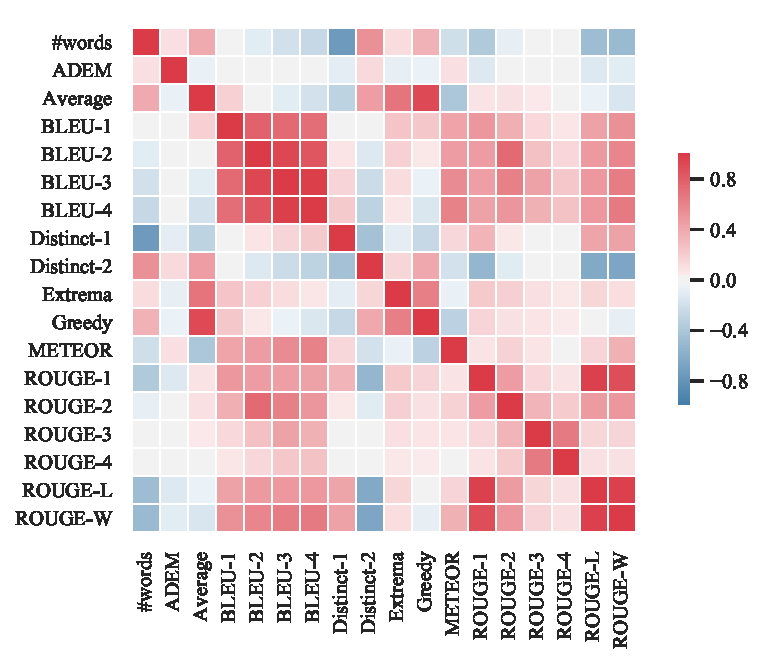
\includegraphics[width=\linewidth]{figure/plot/heatmap/v4/pearson/hred/ubuntu/plot.pdf}
        \caption{(HRED, Ubuntu)}
    \end{subfigure}
    \begin{subfigure}{0.33\linewidth}
        \centering
        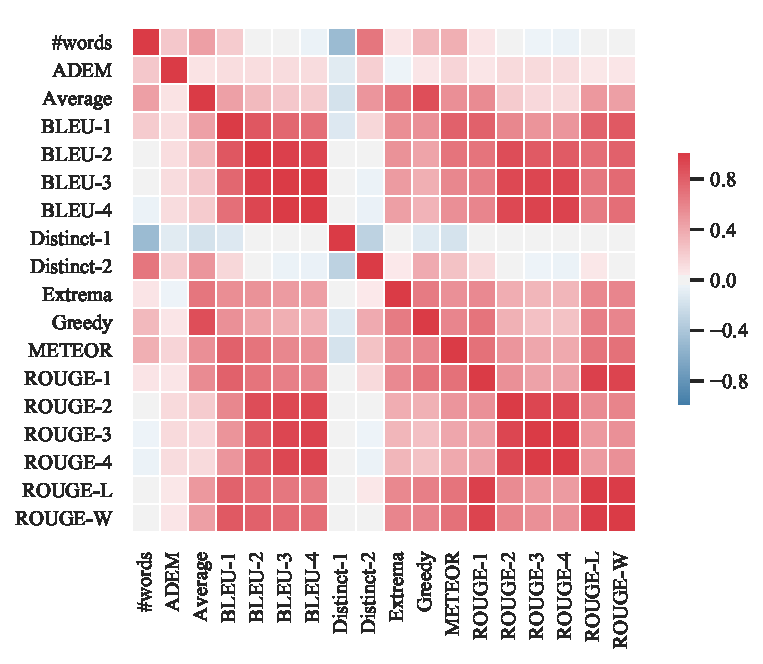
\includegraphics[width=\linewidth]{figure/plot/heatmap/v4/pearson/vhred/lsdscc/plot.pdf}
        \caption{(VHRED, LSDSCC)}
    \end{subfigure}%
    \begin{subfigure}{0.33\linewidth}
        \centering
        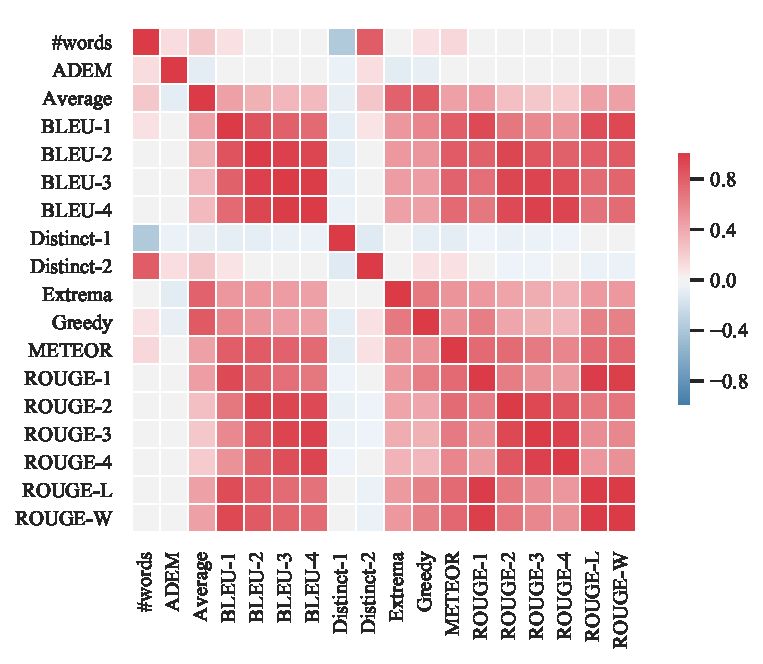
\includegraphics[width=\linewidth]{figure/plot/heatmap/v4/pearson/vhred/opensub/plot.pdf}
        \caption{(VHRED, OpenSubtitles)}
    \end{subfigure}%
    \begin{subfigure}{0.33\linewidth}
        \centering
        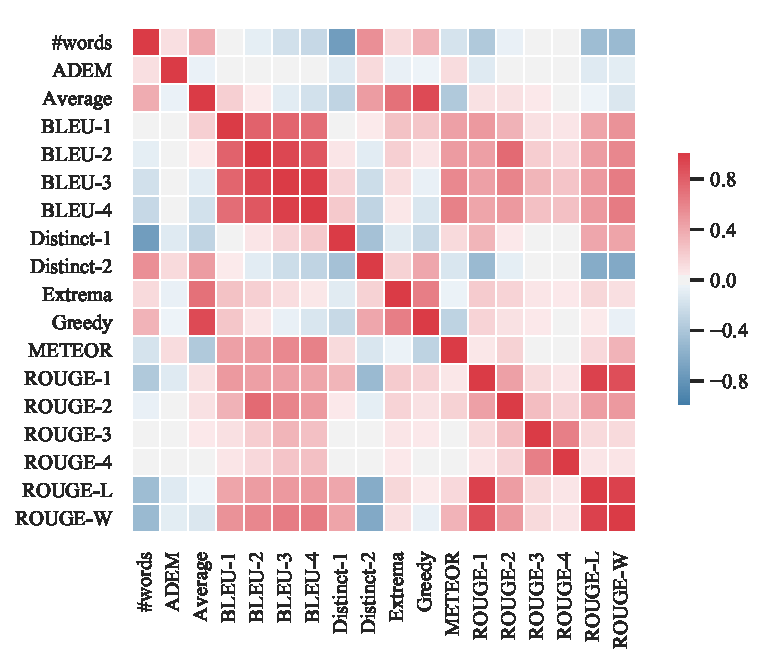
\includegraphics[width=\linewidth]{figure/plot/heatmap/v4/pearson/vhred/ubuntu/plot.pdf}
        \caption{(VHRED, Ubuntu)}
    \end{subfigure}
    \begin{subfigure}{0.33\linewidth}
        \centering
        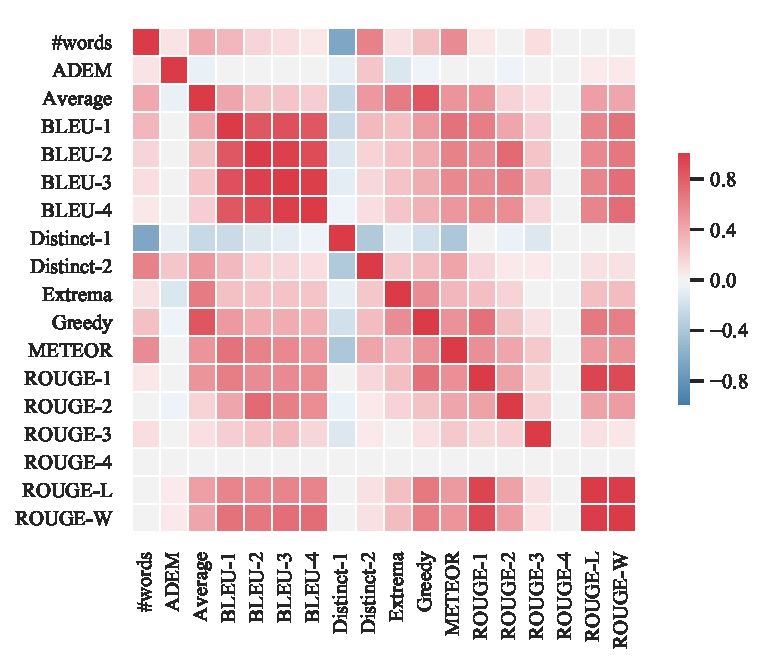
\includegraphics[width=\linewidth]{figure/plot/heatmap/v4/pearson/lstm/lsdscc/plot.pdf}
        \caption{(LSTM, LSDSCC)}
    \end{subfigure}%
    \begin{subfigure}{0.33\linewidth}
        \centering
        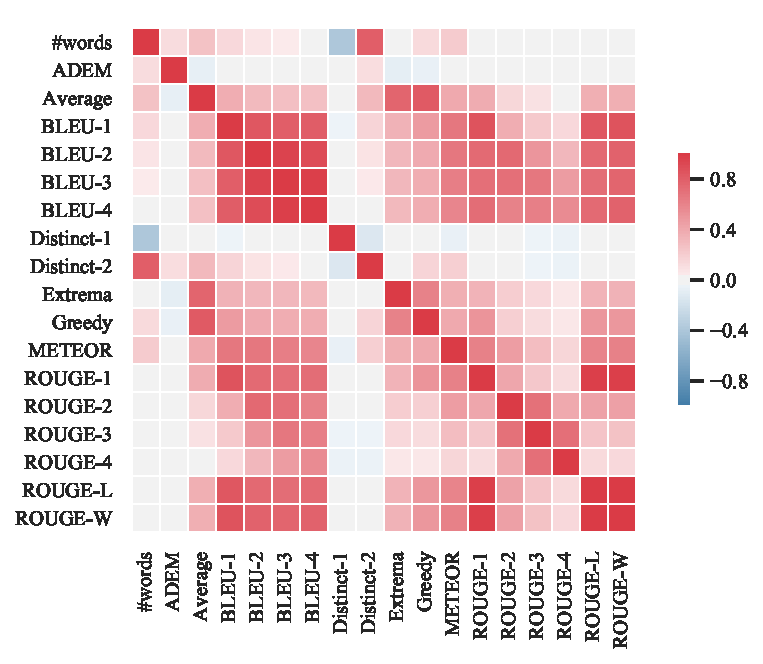
\includegraphics[width=\linewidth]{figure/plot/heatmap/v4/pearson/lstm/opensub/plot.pdf}
        \caption{(LSTM, OpenSubtitles)}
    \end{subfigure}%
    \begin{subfigure}{0.33\linewidth}
        \centering
        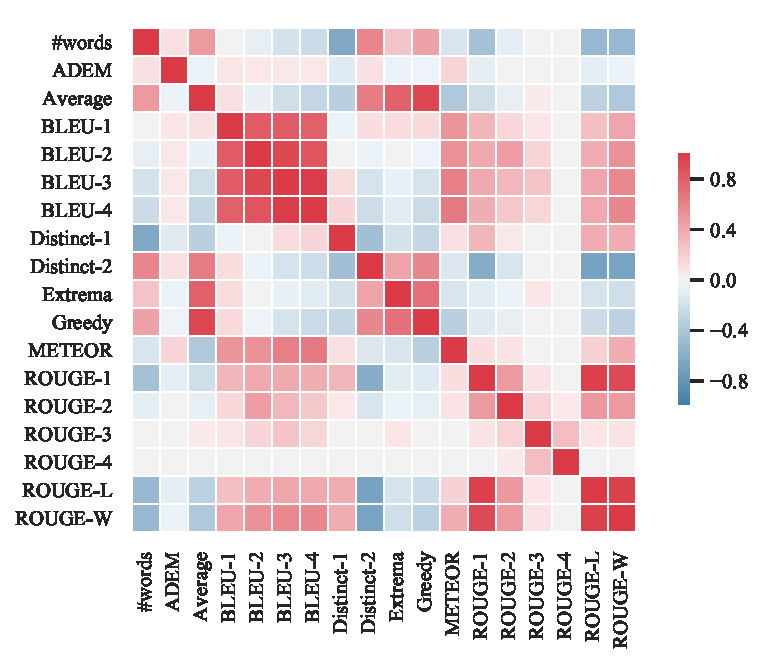
\includegraphics[width=\linewidth]{figure/plot/heatmap/v4/pearson/lstm/ubuntu/plot.pdf}
        \caption{(LSTM, Ubuntu)}
    \end{subfigure}
    \caption{Heatmaps of Pearson's r}
    \label{fig:corr_heatmap}
\end{figure}


Each subfigure in Fig.~\ref{fig:corr_heatmap} was plotted from the correlation matrix for a model instance.
The color of the cells represents the degree of correlation between the row and column labels, with red, blue, and white stand for positive, negative and zero correlation, respectively.
One can observe red regions divided by white or blue lines from these plots, showing the signs of clustering.

To better observe the degree of correlations among different metrics, we applied hierarchical clustering to the metrics based on their correlations and the results are shown in Fig.~\ref{fig:hierarchy}.
A hierarchical clustering algorithm starts with a forest of nodes and iteratively merges them into larger clusters until the root cluster is created.
We used the following node-level distance $\textit{dist}(\cdot, \cdot)$ and cluster-level distance $d(\cdot, \cdot)$:
\begin{align}
    \textit{dist}(i, j) &= 1 - \textit{corr}(i, j) \\
    d(u, v) &= \frac{\sum_{i,j}\textit{dist}(i, j)}{|u| \cdot |v|}
\end{align}
where $i$ and $j$ are points in cluster $u$ and $v$, respectively. $|u|$ and $|v|$ are the cardinalities of cluster $u$ and $v$, respectively\footnote{This is also known as the average method.}. Again the correlation is based on Pearson's r.
\begin{figure}[htb]
    \begin{subfigure}{0.35\linewidth}
        \centering
        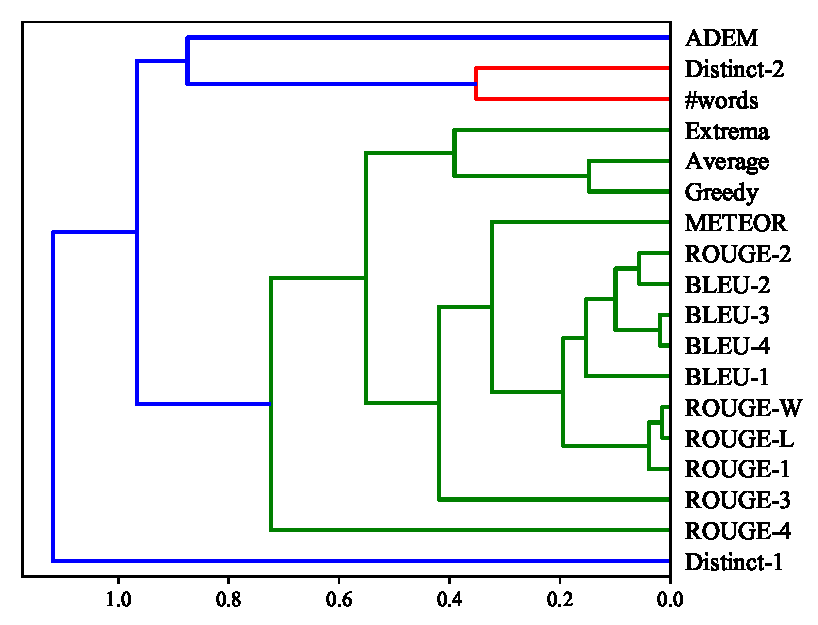
\includegraphics[width=\linewidth]{figure/plot/hierarchy/v3/pearson/hred/lsdscc/plot.pdf}
        \caption{(HRED, LSDSCC)}
    \end{subfigure}%
    \begin{subfigure}{0.35\linewidth}
        \centering
        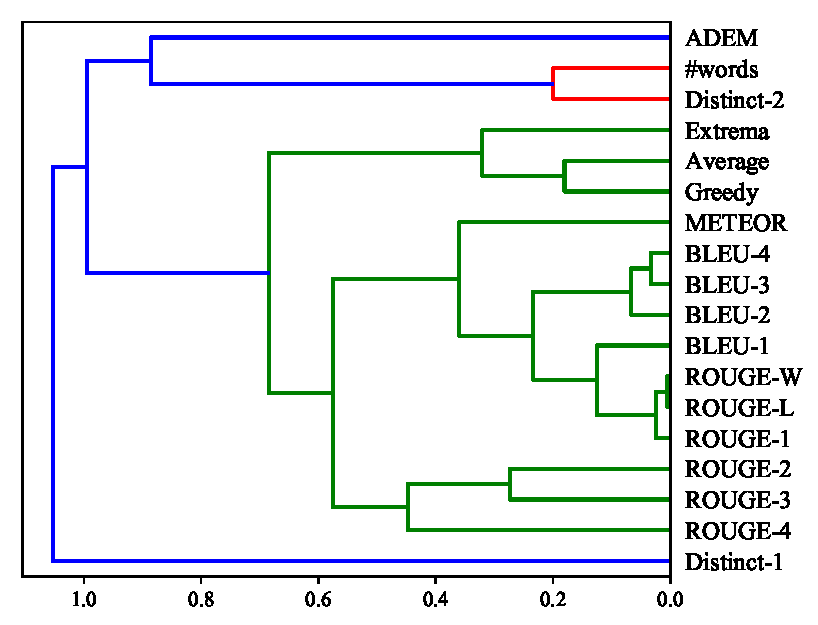
\includegraphics[width=\linewidth]{figure/plot/hierarchy/v3/pearson/hred/opensub/plot.pdf}
        \caption{(HRED, OpenSubtitles)}
    \end{subfigure}%
    \begin{subfigure}{0.35\linewidth}
        \centering
        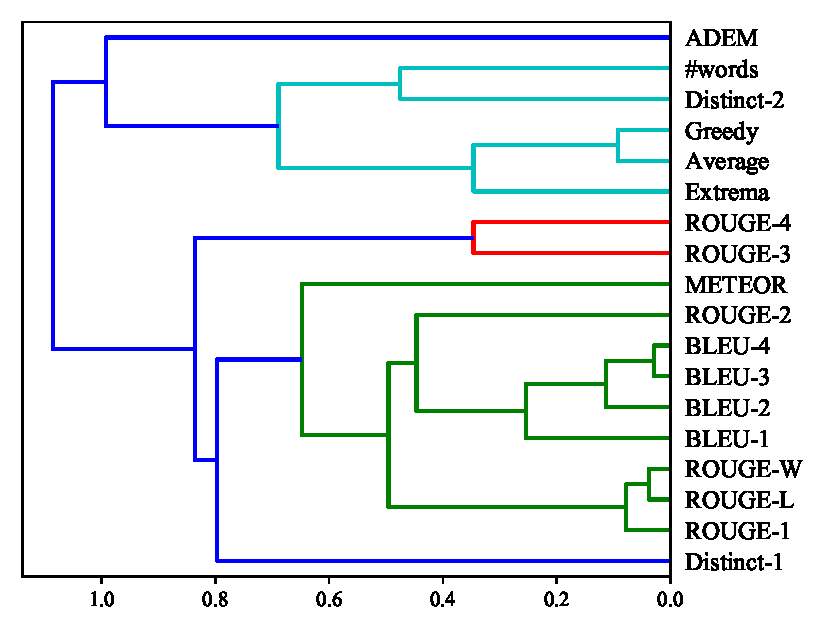
\includegraphics[width=\linewidth]{figure/plot/hierarchy/v3/pearson/hred/ubuntu/plot.pdf}
        \caption{(HRED, Ubuntu)}
    \end{subfigure}
    \begin{subfigure}{0.35\linewidth}
        \centering
        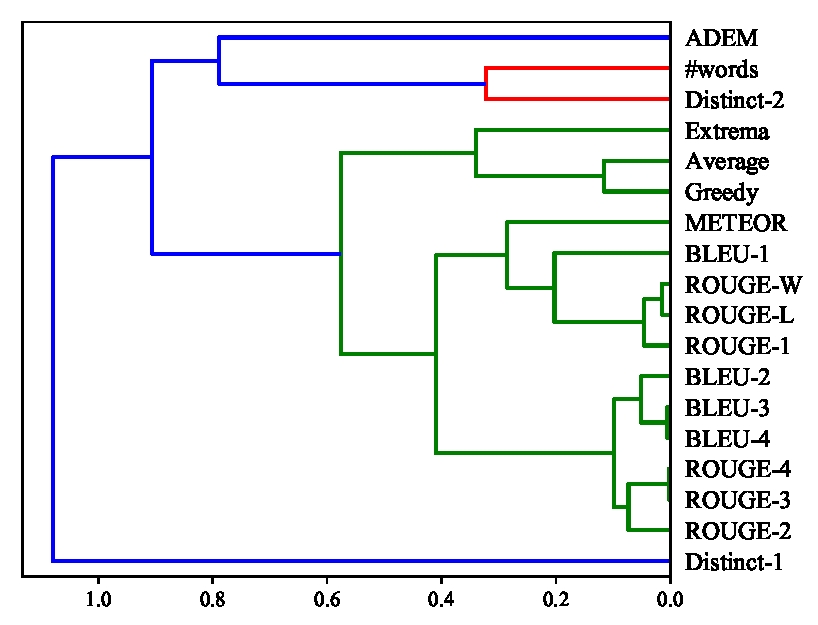
\includegraphics[width=\linewidth]{figure/plot/hierarchy/v3/pearson/vhred/lsdscc/plot.pdf}
        \caption{(VHRED, LSDSCC)}
    \end{subfigure}%
    \begin{subfigure}{0.35\linewidth}
        \centering
        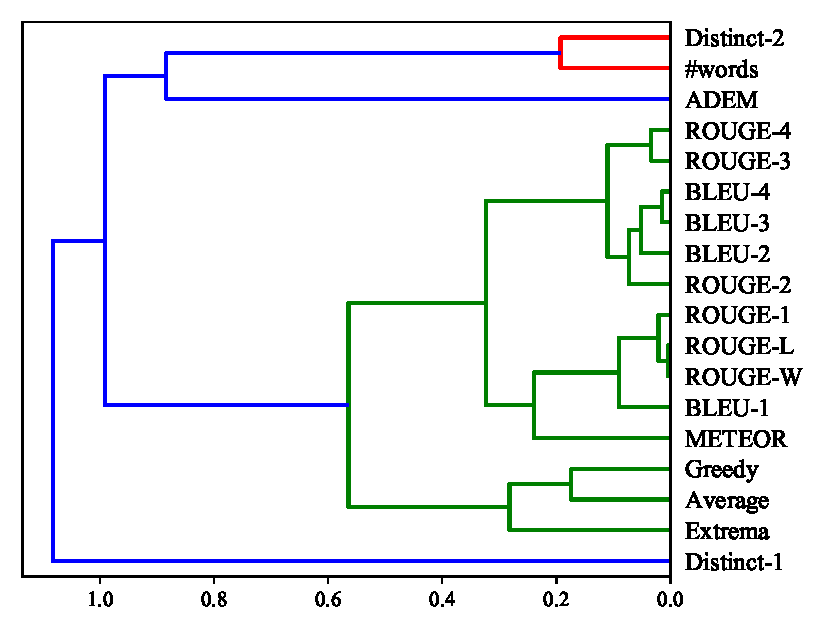
\includegraphics[width=\linewidth]{figure/plot/hierarchy/v3/pearson/vhred/opensub/plot.pdf}
        \caption{(VHRED, OpenSubtitles)}
    \end{subfigure}%
    \begin{subfigure}{0.35\linewidth}
        \centering
        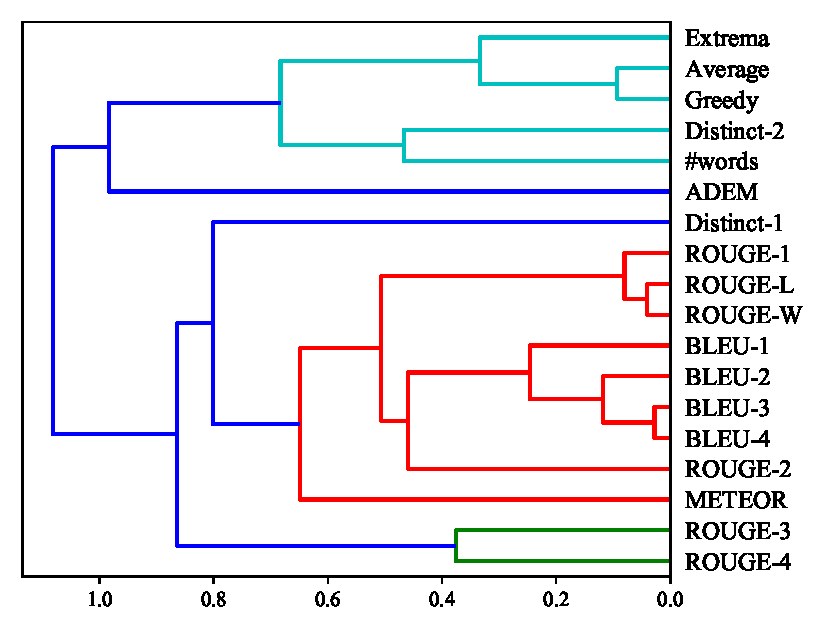
\includegraphics[width=\linewidth]{figure/plot/hierarchy/v3/pearson/vhred/ubuntu/plot.pdf}
        \caption{(VHRED, Ubuntu)}
    \end{subfigure}
    \begin{subfigure}{0.35\linewidth}
        \centering
        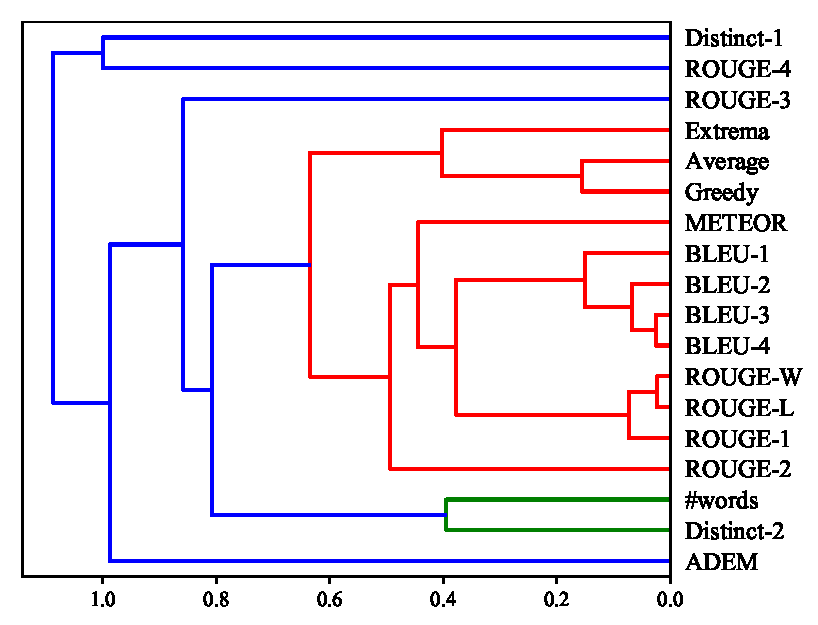
\includegraphics[width=\linewidth]{figure/plot/hierarchy/v3/pearson/lstm/lsdscc/plot.pdf}
        \caption{(LSTM, LSDSCC)}
    \end{subfigure}%
    \begin{subfigure}{0.35\linewidth}
        \centering
        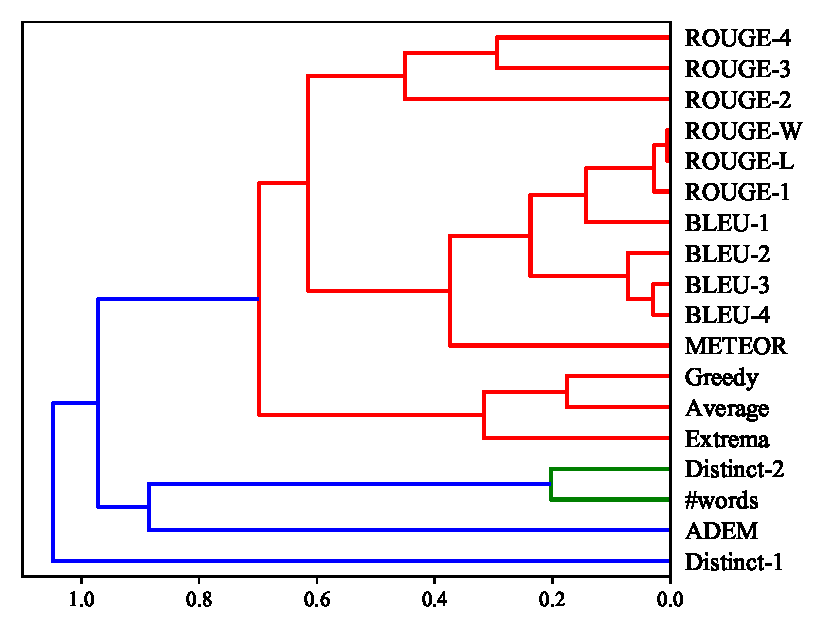
\includegraphics[width=\linewidth]{figure/plot/hierarchy/v3/pearson/lstm/opensub/plot.pdf}
        \caption{(LSTM, OpenSubtitles)}
    \end{subfigure}%
    \begin{subfigure}{0.35\linewidth}
        \centering
        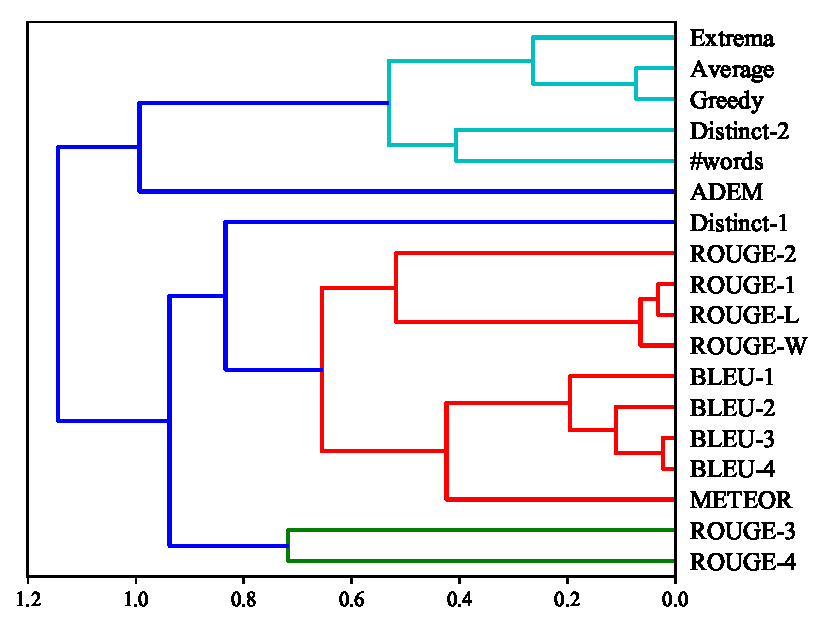
\includegraphics[width=\linewidth]{figure/plot/hierarchy/v3/pearson/lstm/ubuntu/plot.pdf}
        \caption{(LSTM, Ubuntu)}
    \end{subfigure}
    \centering
    \caption{Hierarchical Clusterings with Pearson's r}
    \label{fig:hierarchy}
\end{figure}


From Fig.~\ref{fig:hierarchy}, we observe a hierarchy of agreement among different metrics.
The clusters created in the earlier iterations appear closer to the leaves of the tree, which indicates higher pairwise correlations or stronger inter-metric agreement.
As a cluster grows larger, its children become more loosely connected with greater distances.
It is interesting to find that the dendrograms in Fig.~\ref{fig:hierarchy} share some regular structure, which has a clear correspondence to the category of the metrics. Across all the configurations, we generally observe these independent clusters, named after the shared category or representative element:

1) Word-Overlap: a large cluster that contains many subclusters formed by different word-overlap metrics, such as BLEU, ROUGE, and METEOR.

2) Word-Embedding: a small cluster that contains Vector-Average, Vector-Extrema, and Greedy-Matching.

3) ADEM: a standalone cluster formed by the ADEM metric.

4) Distinct-1: a metric that might belong to some cluster or become a standalone cluster depending on the dataset involved.

5) Distinct-2 and \#words: a generally observable cluster.

Those clusters confirm our hypothesis on the inconsistency among different metrics.
Luckily, there are still some forms of agreement that the same cluster of metrics can reach.
Unfortunately, the exact reasons why the clusters are formed this way are unclear to us.
Although our experiments have a simple procedure, it should be noted that the mechanism behind each step has a complex nature.
For example, the dialogue datasets are intrinsically very diverse and the way the generative models work is not well-understood.
Besides, it is also unclear how these metrics reflect the desirable properties of a response.
Hence we can only conclude that similar metrics tend to have consistent results on the example-level.
The similarity of metrics generally refers to their mechanisms, such as the way to extract overlap units or derive semantics from an utterance, or the way to combine different components.

Specifically, we find that metrics based on word overlap tend to have high pairwise correlations since they all make use of the n-gram statistics in some way.
We also find that ADEM does not correlate well with all the other metrics since it has a much higher correlation with human judgement while other metrics do not.

\subsection{Qualitative Analysis}
\begin{table*}
    \caption{An Example from OpenSubtitles}
    \label{tab:AnExampleFromOpenSubtitles}
    \centering
    \begin{tabular}{|l|*{3}{p{0.2\textwidth}|}}
        \hline
        Context & \multicolumn{3}{p{0.64\textwidth}|}{you il be in classes does she know that ? </s> as if you re gonna have all this free time to pal around with her </s>} \\
        \hline
        Reference & \multicolumn{3}{p{0.64\textwidth}|}{okay sure we il start there </s>} \\
        \hline
        Model & LSTM & HRED & VHRED \\
        \hline
        Response & c all this time & her room starts in half 50 percent & i figured this was gonna be a fun stretch \\
        \hline
        ADEM & 2.5987 & \textbf{2.6411} & 2.6276 \\
        \hline
        BLEU-1 & 0 & 0 & 0 \\
        \hline
        Distinct-1 & 1.0 & 1.0 & 1.0 \\
        \hline
        Distinct-2 & 0.75 & 0.8571 & \textbf{0.8889} \\
        \hline
        Greedy & \textbf{0.3520} & 0.2336 & 0.3412 \\
        \hline
        Average & 0.4979 & 0.3468 & \textbf{0.6607} \\
        \hline
        Extrema & 0.2791 & 0.1341 & \textbf{0.3995} \\
        \hline
        METEOR & 0 & \textbf{0.0105} & 0 \\
        \hline
        ROUGE-L & 0 & 0 & 0 \\
        \hline
        ROUGE-W & 0 & 0 & 0 \\
        \hline
        \#words & 4 & 7 & \textbf{9} \\
        \hline
    \end{tabular}
\end{table*}

Table~\ref{tab:AnExampleFromOpenSubtitles} serves as an instance of the example-level inconsistency of metrics
\footnote{The symbol $</s>$ denotes the end of a sentence.}.
The context conveys the fact that ``you'' will be in the same class with ``her''
and assumes that ``you'' will have plenty of time to play together with ``her''.
The reference is a positive reply to the context.

The response from HRED mentions ``her room'', which is relevant to the subject ``she'' in the context and the verb ``starts'' matches the ``start'' in the reference.
The response from VHRED does not share any word with the context or reference, but it makes a positive comment on the fact, which is most appropriate one among the three.
The response from LSTM is not a complete sentence and its meaning is unclear.

% Note: Three responses share n-grams with context, but not reference.
All three responses share no n-grams with the reference so all the word-overlap metrics yield a zero value.
However, all the word-embedding metrics give non-zero value, making them inconsistent with the word-overlap metrics.

In terms of topic relevance, the responses from HRED and VHRED are strongly related to the topic of the dialogue, while the response from LSTM is off-topic.
However, the ranks given by the word-embedding metrics do not agree with our manual inspection.
Greedy and Average both give highest scores to LSTM, while Extrema gives lowest score to HRED.
The inconsistent scores cannot reflect the quality of the responses.

\section{Conclusion and Future Work}
% Summary of the experiment results.
In this paper, we follow the work of \cite{HowNot} and try to understand the reasons behind low metric-human correlations.
We perform statistical analyses on both the system-level scores and example-level scores on three commonly used models and datasets.
Our experiments show that while the system-level scores are relatively consistent in terms of the best model,
the example-level scores are only consistent within the same group of metrics.
As each metric may introduce their own bias into the evaluation process, their scores are potentially inconsistent by nature.
However, these inconsistencies may counteract each other when being summed up so the system-level scores still look consistent.
The inconsistency between different evaluation metrics may contribute to the low human-metric correlation.

% Recommendations based on the experiments.
Based on the experiment results, it is advised to avoid evaluating generative models with a single metric as the results may not be
consistent with alternative metrics. Besides, human judgements should be consulted when possible since
the metrics are known to be inconsistent and may mislead the direction of fine-tuning.

% Future direction of developing better metrics.
To develop better metrics, it is advised to consider the example tuple $(context, reference, response)$
as a whole and pay attention to both the intrinsic properties of a response (i.e., its grammatical correctness, fluency etc.) and its relationships to the context and reference (i.e., topic relevance, engagement etc.). It is also advised to use human judgements data as supervised signals to refine evaluation metrics, as in \cite{ADEM}.

% Our future work.
It is widely acknowledged that human judgements are indispensable for the evaluation of generative models.
In the future, we would like to introduce human scores as a baseline and directly compute their correlations with metrics.
Although hierarchical clusters of metrics are observed in this research, it is not clear whether this is a general phenomenon for evaluation metrics.
In the future, we would like to deepen our understanding on the mechanisms behind the scene.
We would also like to include more recently proposed evaluation methods to make our survey more comprehensive.

\section*{Acknowledgments}
This work was partially supported by the State Key Laboratory of Software Development Environment of China (No. SKLSDE-2019ZX-15).

% trigger a \newpage just before the given reference
% number - used to balance the columns on the last page
% adjust value as needed - may need to be readjusted if
% the document is modified later
%\IEEEtriggeratref{8}
% The "triggered" command can be changed if desired:
%\IEEEtriggercmd{\enlargethispage{-5in}}

% references section

% can use a bibliography generated by BibTeX as a .bbl file
% BibTeX documentation can be easily obtained at:
% http://www.ctan.org/tex-archive/biblio/bibtex/contrib/doc/
% The IEEEtran BibTeX style support page is at:
% http://www.michaelshell.org/tex/ieeetran/bibtex/
%\bibliographystyle{IEEEtran}
% argument is your BibTeX string definitions and bibliography database(s)
%\bibliography{IEEEabrv,../bib/paper}
%
% <OR> manually copy in the resultant .bbl file
% set second argument of \begin to the number of references
% (used to reserve space for the reference number labels box)
% control reference type settings
\balance

\bibliographystyle{IEEEtran}
\bibliography{reference}

% that's all folks
\end{document}
